\begin{frame}\frametitle{\vspace*{0.5cm}I plan to increase the relevance to DUS}
  Hypothesis: Baroclinic vorticity drives deformation to the point of
  stress or strain failure in pulmonary capillaries.
  % 
  \begin{itemize}
  \item Rabbit pulmonary capillaries have been shown to hemorrhage at transmural stresses of $\approx 5$ kPa \citep{West1991}.
  \item I will calculate elastic and (passive) viscous stresses at the interface.\vfill%
    \vspace*{5pt}
  \end{itemize}
  % 
  \begin{figure}
    \centering
    \def\svgwidth{0.4\textwidth}%
    {\tiny
      \import{./figs/}{usbe_lung_model_arclength.pdf_tex}%
    }
  \end{figure}
  %
\end{frame}

\begin{frame}\frametitle{\vspace*{0.5cm}I plan to increase the relevance to DUS}
  Hypothesis: vorticity induced deformation and subsequent hemorrhage will allow acoustic waves and hemorrhage to propagate into
  subsequent layers of alveoli\\
  \begin{itemize}
  \item Damage exists in clearly defined hemorrhage area, not behind it \citep{Penney1993a}.
  \item Propagation mechanism of US-induced lesions are unknown \citep{Zachary2006}.
  \end{itemize}
  \begin{figure}
    \centering
    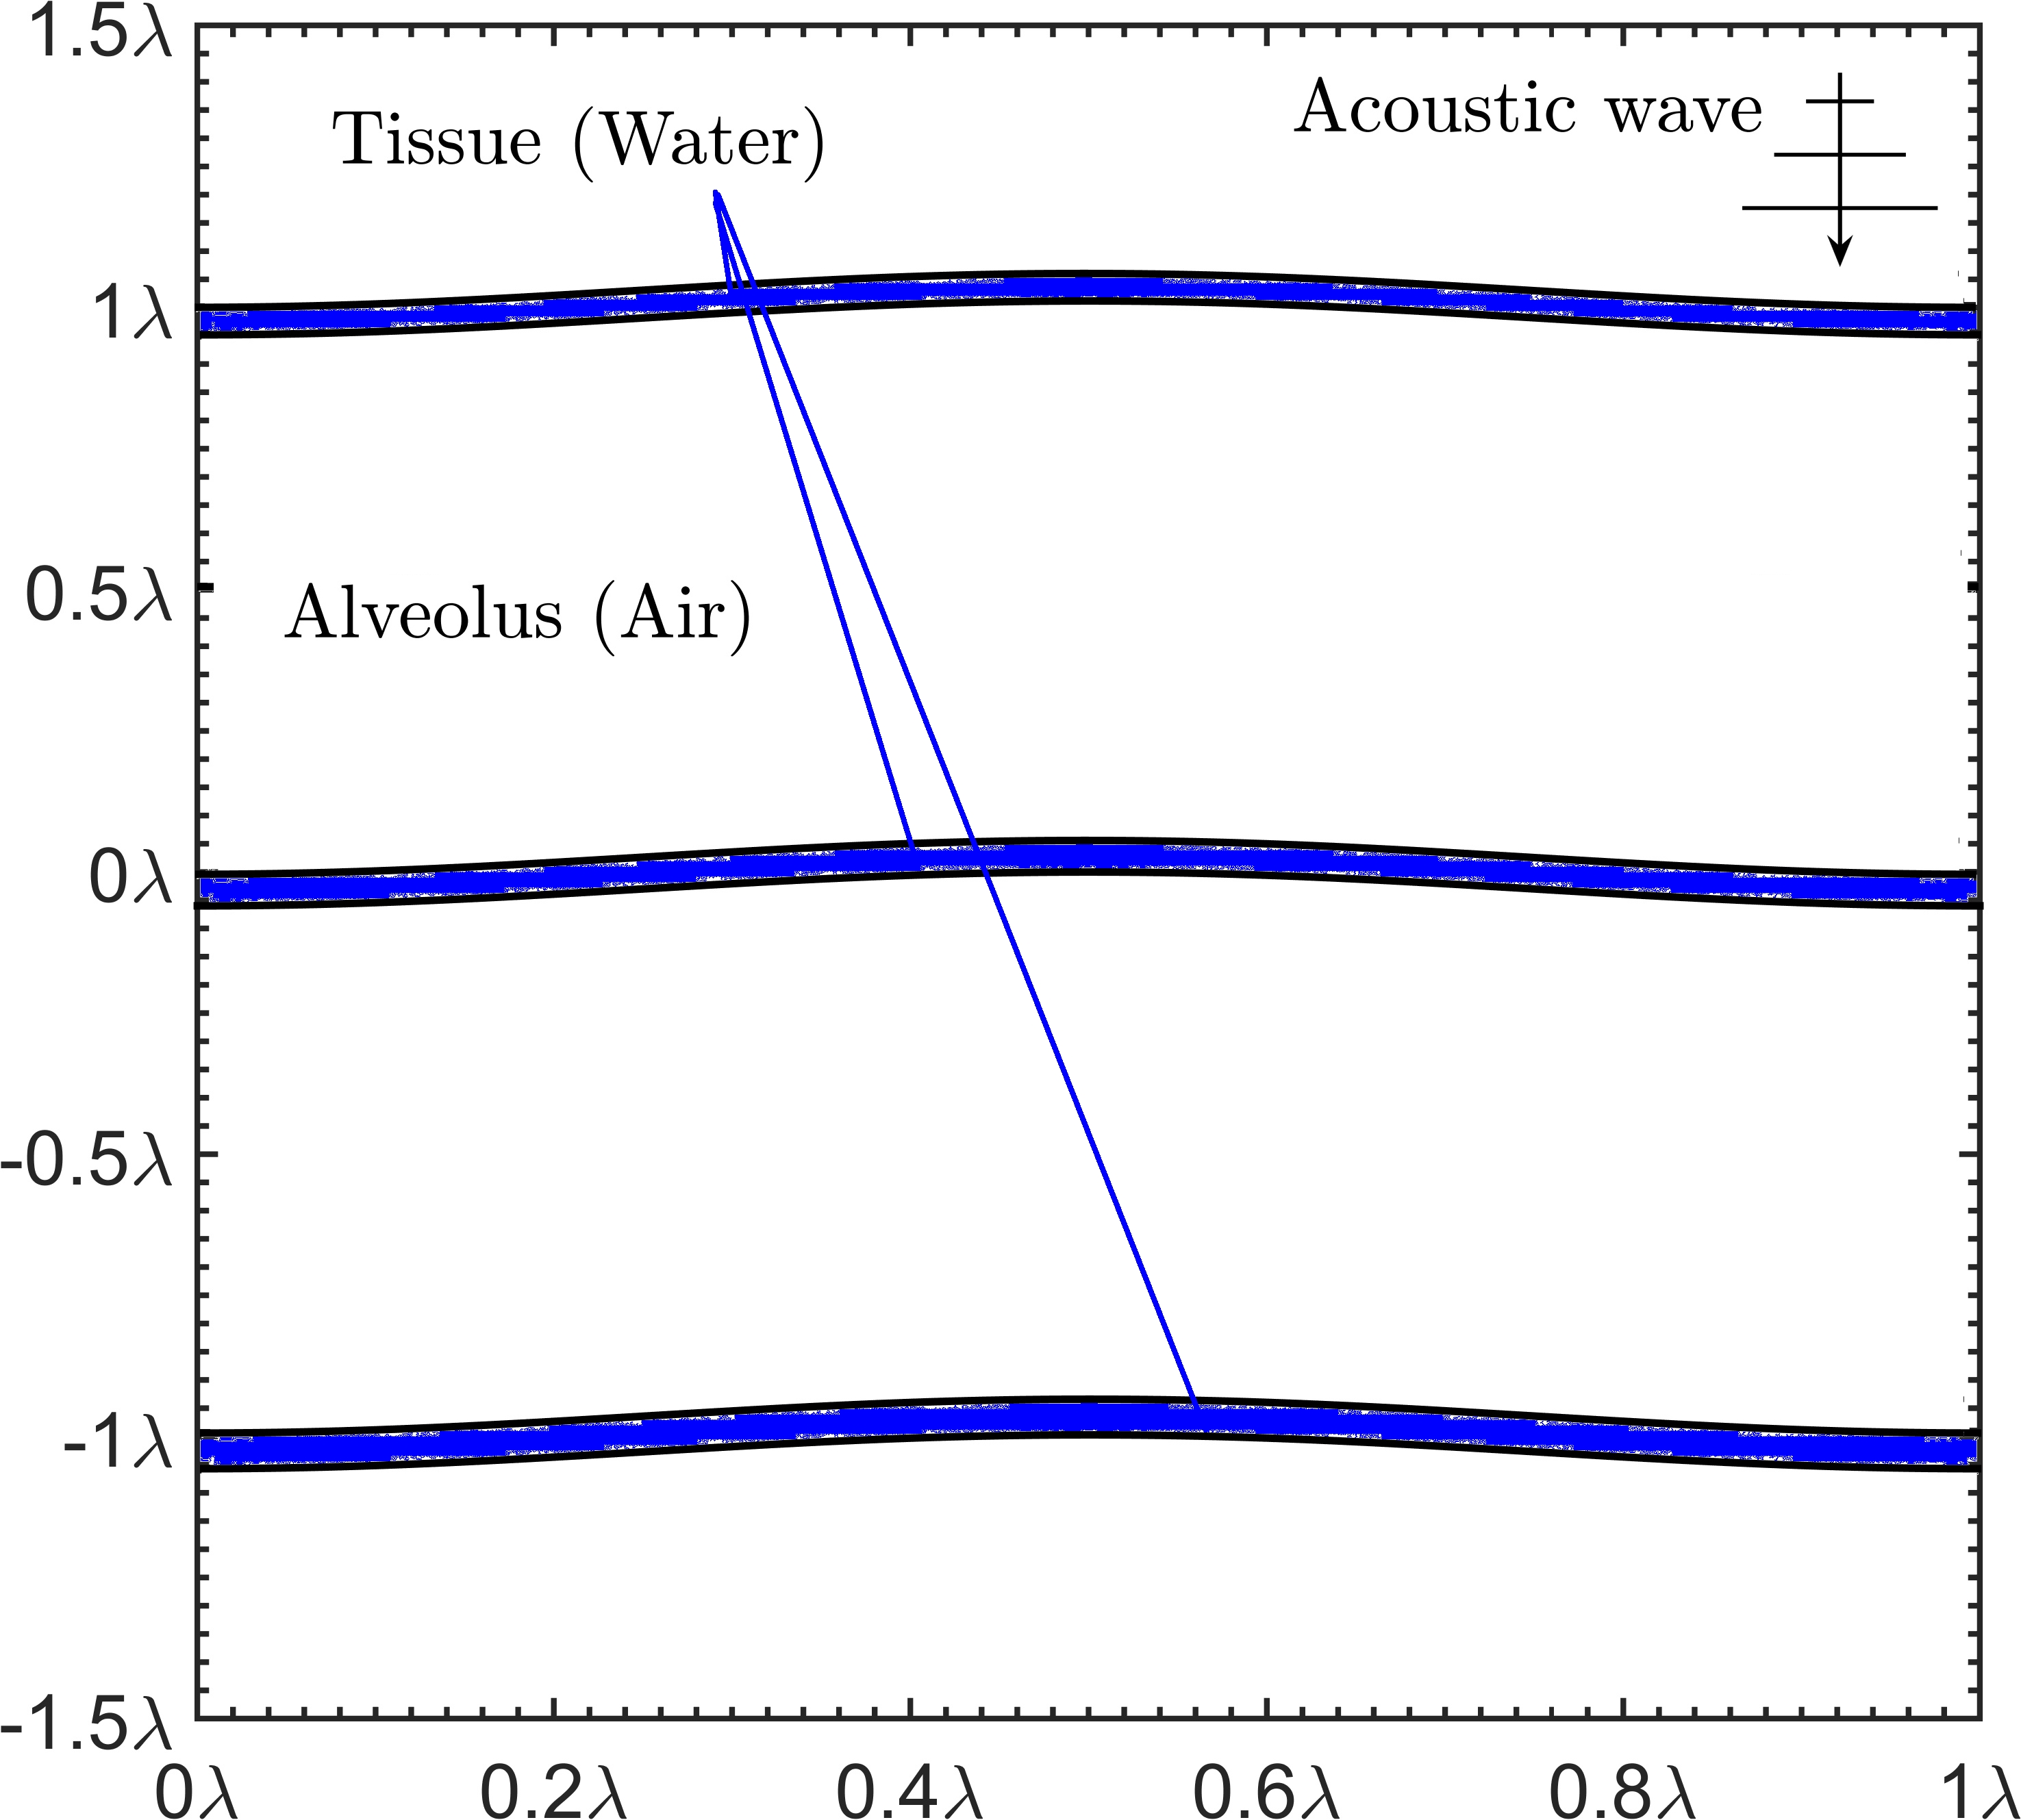
\includegraphics[width=0.5\textwidth]{../figs/lung_figs/usbe_model_schematic_periodic}
  \end{figure}
  \note{Mauro's Question:
    (1) Would a bubble-like configuration be more relevant/useful?
  }
\end{frame}

\begin{frame}\frametitle{Future work (beyond me)}
  To fully understand the role that fluid mechanics plays in DUS-induced lung hemorrhage, the following problems need to be addressed:\\
  \vspace*{0.25cm}
  \begin{itemize}
  \item Viscous effects\vfill%
  \item Elasticity and failure mechanics\vfill%
  \item Multiple pulses (via time-dependent boundary conditions)\vfill%
  \item Detailed pulmonary structure\vfill%
  \end{itemize}
\end{frame}
%
%%% Local Variables:
%%% mode: latex
%%% TeX-master: "../main"
%%% End:
